\documentclass[openany]{article}

%Standard Stefanos Packages
\usepackage[utf8]{inputenc}
\usepackage{dirtytalk}
\usepackage{amsmath}
\usepackage{mathtools}  
\mathtoolsset{showonlyrefs} 
\usepackage{graphicx}
\usepackage{mdframed}
\usepackage{lipsum}
\usepackage{cancel}
\usepackage{systeme}
\usepackage{pgfplots}
\usepackage{textcomp}
\usepackage{geometry}
\usetikzlibrary{arrows}
\geometry{a4paper}
\graphicspath{ {./res/} }
\usepackage{float}
\restylefloat{table}
\newcommand{\comment}[1]{%
	\text{\phantom{(#1)}} \tag{#1}
}
\title{\line(3,0){250}\\PROGRAMMING IN PYTHON FOR DATA SCIENCE(CS3PP19) \\ Final Exam: Question 1  \\\line(3,0){250}}
\usepackage{pgfplots}
\author{52944}
\newmdtheoremenv{note}{Note}
\pgfplotsset{compat=1.17}


%Extra Packages
\usepackage{tikz}
\usetikzlibrary{automata,positioning}

\usepackage{listings}
\usepackage{xcolor}

\definecolor{dkgreen}{rgb}{0,0.6,0}
\definecolor{gray}{rgb}{0.5,0.5,0.5}
\definecolor{mauve}{rgb}{0.58,0,0.82}

\lstdefinestyle{myScalastyle}{
	frame=tb,
	language=scala,
	aboveskip=3mm,
	belowskip=3mm,
	showstringspaces=false,
	columns=flexible,
	basicstyle={\small\ttfamily},
	numbers=none,
	numberstyle=\tiny\color{gray},
	keywordstyle=\color{blue},
	commentstyle=\color{dkgreen},
	stringstyle=\color{mauve},
	frame=single,
	breaklines=true,
	breakatwhitespace=true,
	tabsize=3,
}

\begin{document}
	\maketitle
	\section{Initialization Code}
	\begin{lstlisting}[language=Python]
import pandas as pd
from pandas.plotting import parallel_coordinates
data=pd.read_csv("data.csv")
data=data.dropna()
	\end{lstlisting}
	\section{Q1.a.i}
		\begin{lstlisting}[language=Python]
def top_publishers(df_input,att,top_num):
	return df_input[[att,"Publisher"]]\
		.groupby("Publisher")\
		.sum()\
		.sort_values(att,ascending=False)[:top_num]

		\end{lstlisting}
	\section{Q1.a.ii}
		\begin{lstlisting}[language=Python]
top5=top_publishers(data,"Global_Sales",5)
top5.plot.bar()
		\end{lstlisting}
		\begin{figure}[H]
			\iftrue
			\centering
			\caption{Global sales trend amongst 5 top publishers}
			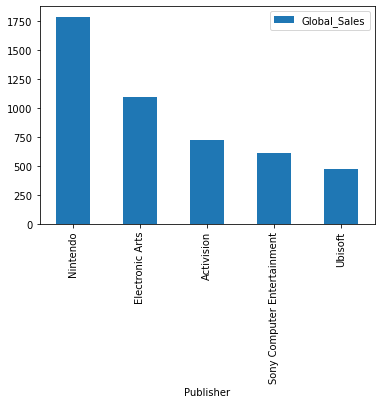
\includegraphics[scale=0.5]{global-sales-trend}
			\fi
		\end{figure}
	\section{Q1.a.iii}
		\subsection{Process the data to show in one graph the total sales pergeographic area (e.g. North America, Europe, etc.).}
			\begin{lstlisting}[language=Python]
pd.DataFrame({
	"NORTH AMERICA":[data.NA_Sales.sum()],
	"EUROPE":[data.EU_Sales.sum()],
	"JAPAN":[data.JP_Sales.sum()],
	"OTHER":[data.Other_Sales.sum()]}).plot.bar()
			\end{lstlisting}
			\begin{figure}[H]
				\iftrue
				\centering
				\caption{Global sales trend amongst 5 top publishers}
				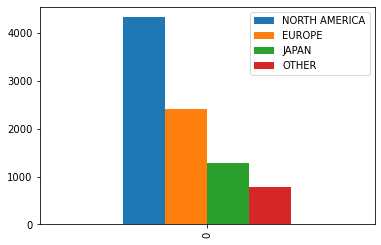
\includegraphics[scale=0.5]{sum-sales-per-region}
				\fi
			\end{figure}	
		\subsection{How is the sales distribution in these markets divided considering the top 5 publishers in global sales?}
			\begin{lstlisting}[language=Python]
sales_data=data.loc[
	(data["Publisher"].isin(list(top5.reset_index()["Publisher"])))]\
	.groupby("Publisher")\
	.sum()
parallel_coordinates(\
	sales_data[["NA_Sales","EU_Sales","JP_Sales","Other_Sales"]]\
	.reset_index(),"Publisher")

			\end{lstlisting}
			\begin{figure}[H]
				\iftrue
				\centering
				\caption{sales per region amongst 5 top publishers}
				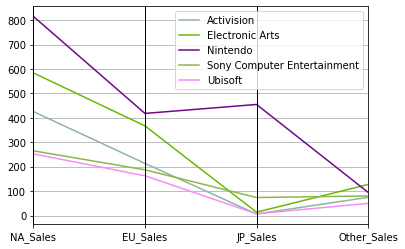
\includegraphics[scale=0.5]{top5-sales-per-region-par}
				\fi
			\end{figure}
		\subsection{Q1.b}
			Our strategy of curating the dataset before starting a data science project relies heavily on the project's requirements. 
			As there are no requirements given, I will briefly explain the standard steps that need to be taken. Finally, I will demonstrate 
			some use cases and provide steps for those.
			\subsubsection{Standard Preproccessing}
				There are several steps considered as a standard before any data science algorithm is applied to the dataset. These are ...
			\begin{itemize}
				\item Dropping the rows containing missing values with .dropna() (dataset is large enough so dropping columns is not an issue)
				\item Year column type should be converted to Integer (for obvious reasons)
				\item Global sales column should be removed, as is highly correlated with the NA,EU,JN,OTHER sales columns(summation)
			\end{itemize}
			\subsubsection{Requirement-specific proccess}
				\begin{itemize}
					\item Given more requirements, domain-specific knowledge may allow us to discard unnecessary columns. 
					For example, in our questions (Q1.a), we perform some EDA around sales. In the specific EDA, the columns Rank, 
					Platform, Year, Gendre could be discarded.
					\item Do we want to find relationships between variables or just summary statistics and complex queries? 
					If our data science project aims to find relationships between different variables, then a normalization-outliers 
					excluding strategy is necessary. In our EDA on question A, such a move was not needed.
				\end{itemize}
				
\end{document}